\section{Running and Creating New Code}
The physical modelica models are the cornerstone of the Hybrid repository. They are designed to represent physical industrial processes that can be configured into different potential integrated energy systems (IES).
Table \ref{tab:table1} gives an overview of the main types of integrated energy systems, along with models currently incorporated in the hybrid repository.


\begin{table}
\begin{center}
\caption{Examples of large-Scale Systems within the Hybrid repository used in the creation of Integrated Energy Systems.}
\label{tab:table1} 
\begin{tabularx}{\columnwidth}{l|X|X} % <-- Alignments: 1st column left, 2nd middle and 3rd right, with vertical lines in between
      \textbf{Category} & \textbf{Description} & \textbf{Specific Example}\\
      \hline
      \textbf{Primary Heat System} & Provides base load heat and power & Nuclear Reactor\\
      \textbf{Energy Manifold} & Distributes thermal energy among subsystems & Steam Manifold\\
      \textbf{Balance of Plant} & Serves as primary electricity supply from energy not used in other subsystems & Turbine, condenser, and feedtrain\\
      \textbf{Industrial Process} & Generates high value product(s) using heat and electricity from other systems & Steam Electrolysis, gas to liquids, reverse osmosis\\
      \textbf{Energy Storage} & Serves as energy buffer to increase overall system robustness and system that can increase profits during highly fluctuating energy prices & Electric Batteries, Two-Tank Sensible Heat Storage, Thermocline \\
      \textbf{Secondary Energy Source} & Delivers small amounts of topping heat required by industrial processes or rapid dynamics in grid demand that cannot be met the remainder of the system & Natural Gas Turbine\\
      \textbf{Switch Yard} & Distributes electricity among subsystems, including the grid & Electricity Distribution \\
      \textbf{Electrical Grid} & Sets the behavior of the grid connected to the IES & Large Grid Behavior\\
      \textbf{Control Center} & Provides proper system control and test scenarios  & Control System/ Supervisory Control System\\
\end{tabularx}
\end{center}

\end{table}




\begin{figure}[hbtp]
\centering
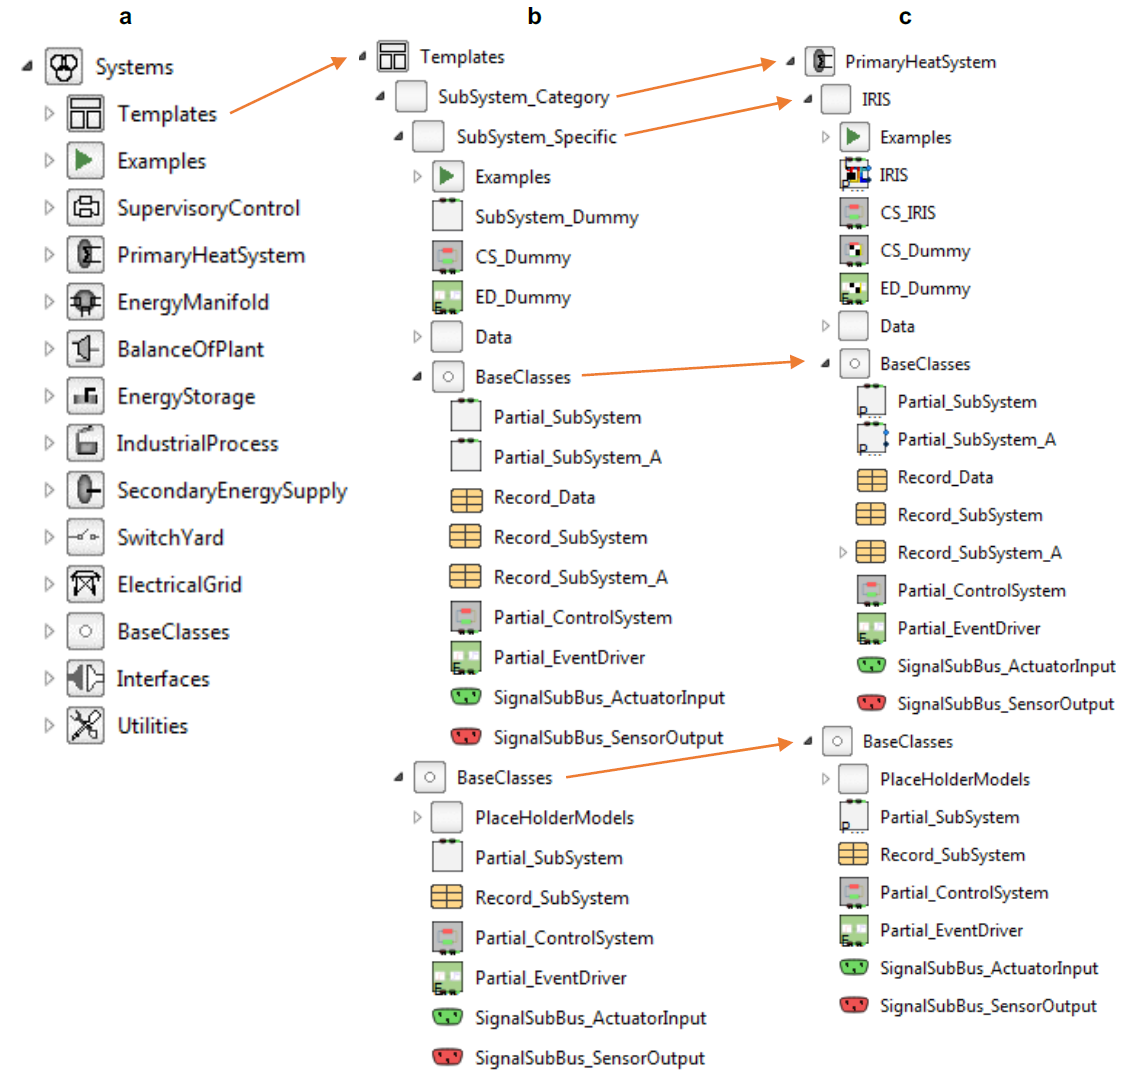
\includegraphics[width=\linewidth]{pics/Template System.png}
\caption{a) Overall Modelica package, b) template structure for creating new subsystem categories and specific subsystem models within a category,  c) example of a specific implementation of a primary heat system using the template approach. }
\label{fig:Template}
\end{figure}



\subsection{Understanding and Running Existing Models}

The hybrid repository is broken down using the templating system shown in Figure \ref{fig:Template}. 
The top level is the overall system package which incorporates all of the Modelica models contained within the NHES package. Then inside of the NHES package are the different subpackages (Systems, Electrical, Thermal, etc…). Within each of the subpackages are further subpackages as seen in the Systems package. Within the Systems package there are further subpackages called \textit{SubSystem Category} (Examples, PrimaryHeatSystem, EnergyStorage, etc…). Then within these SubSystem Categories there is yet another level of subpackage that is called \textit{SubSystem\textunderscore Specific}. Within the \textit{SubSystem\textunderscore Specific} category is where development takes place and potential configurations of the different processes take shape. Inside each SubSystem\textunderscore Specific there is a template that includes \textit{Examples}, \textit{Subsystem Dummy}, \textit{CS\textunderscore Dummy}, \textit{ED\textunderscore Dummy}, Data, BaseClasses, and usually a Components folder. For existing systems the Examples folder contains a runnable example the user can execute to see how the code runs at a top level and what scenarios it is capable of running. An example of which is depicted in Figure \ref{Example File}. For each example the user can double click on the main system which will open the table in the upper left hand corner of Figure \ref{Example File} which provides inputs for the user to change parameters about the system. Then if the user wishes to modify the control system utilized they can either choose from the drop-down menu, or click the button at the right of the “CS” line to open the table in the lower left hand section which provides options to delay when different control systems come online.  

\begin{figure}[hbtp]
\centering
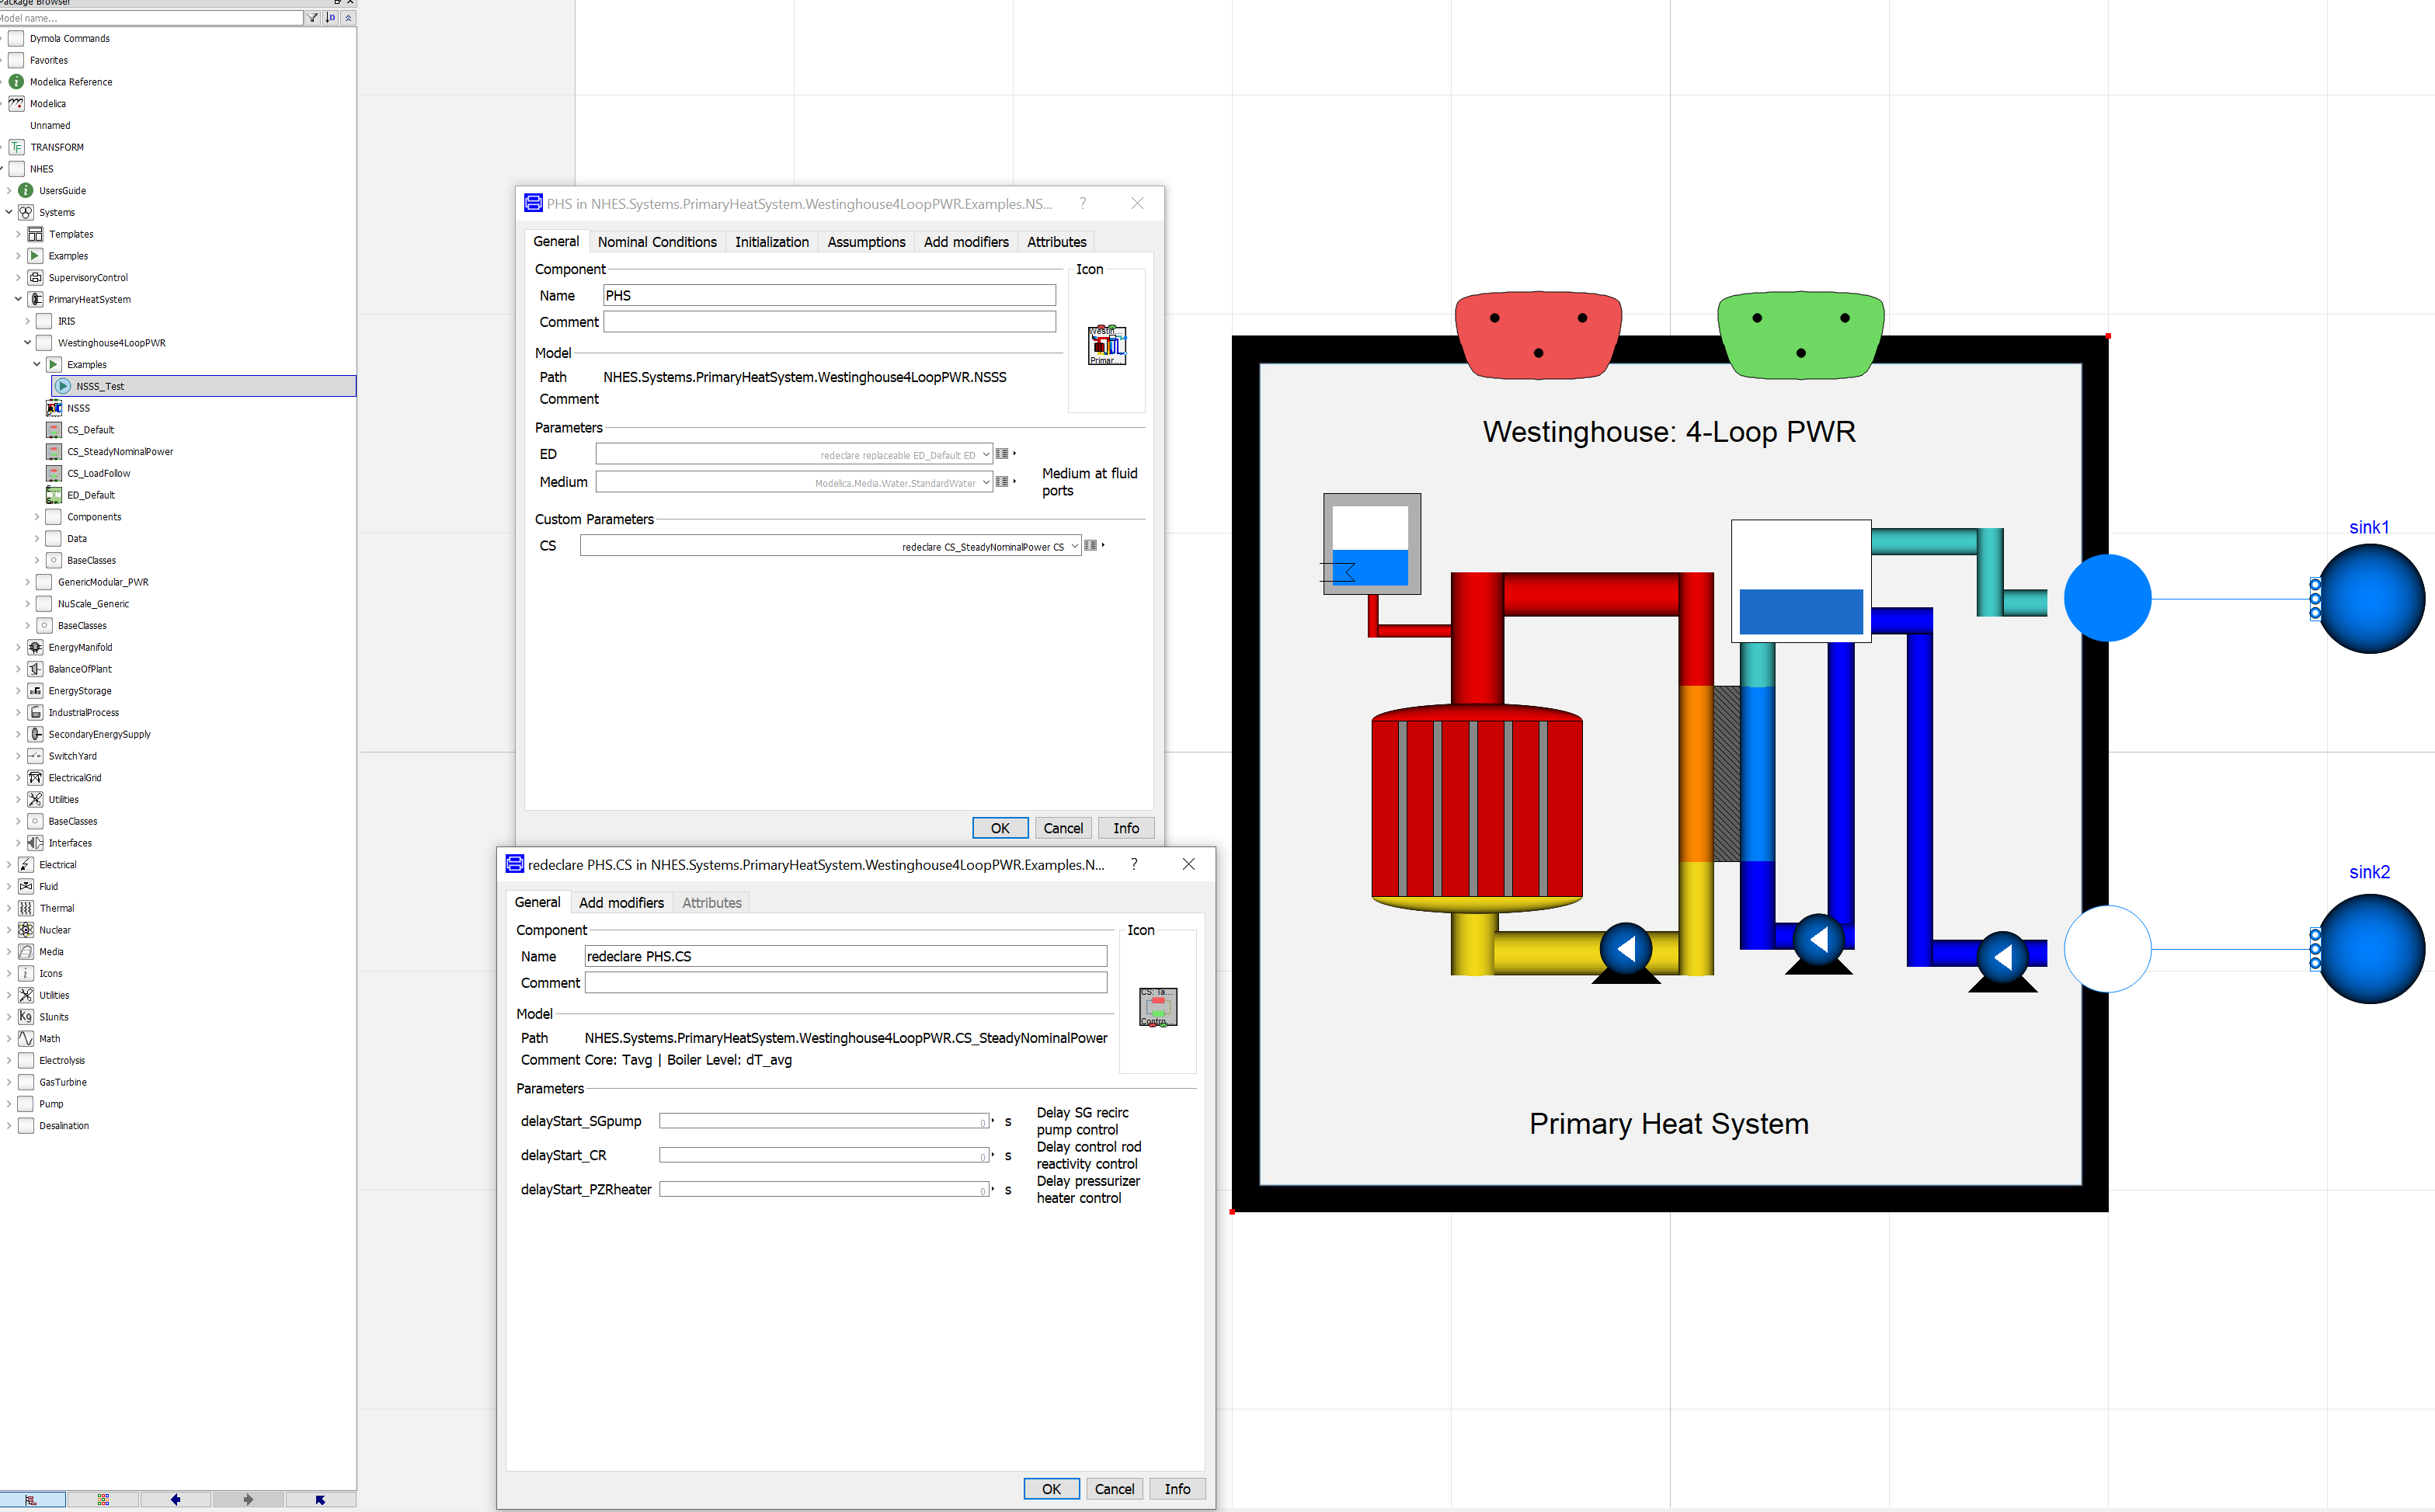
\includegraphics[width=\linewidth]{pics/Example_File.png}
\caption{Exploded view of the NSSS\textunderscore Test example within the NHES library with control system options opened up }
\label{Example File}
\end{figure}

These example tests provide a good way for the user to become associated with the large subsystem in terms of how they work and the different parameters that can be utilized to tune and interact with the models. In addition to the examples file a deeper understanding of the model can be realized by looking into the component structure of the model. This is typically accomplished through looking at the filled-out Subsystem Dummy section. For the Westinghouse 4-Loop plant this can be seen in Figure \ref{Westinghouse 4-loop}. This model includes several subcomponents connected into a singular model. Each model with its’ own set of parameters. Using this version of the model it is possible to discern the inner workings of the model in terms of sensors, physical descriptions of the code, inlet and outlet conditions, and system dependencies. 
In addition to the SubSystem Dummy section, large process models typically include a control system section which is created from the CS\textunderscore Dummy file in the branch. These control system files can be added as a control system for the Subsystem to control different valves, pumps, and control drives within the process from the dropdown menu in the “CS” section seen in Figure \ref{Example File}. large process systems may have several different potential control systems based upon what type of Integrated Energy System they are operating within. An illustration of one of the Westinghouse Control systems can be seen in Figure \ref{Control System}. 


\begin{figure}[hbtp]
\centering
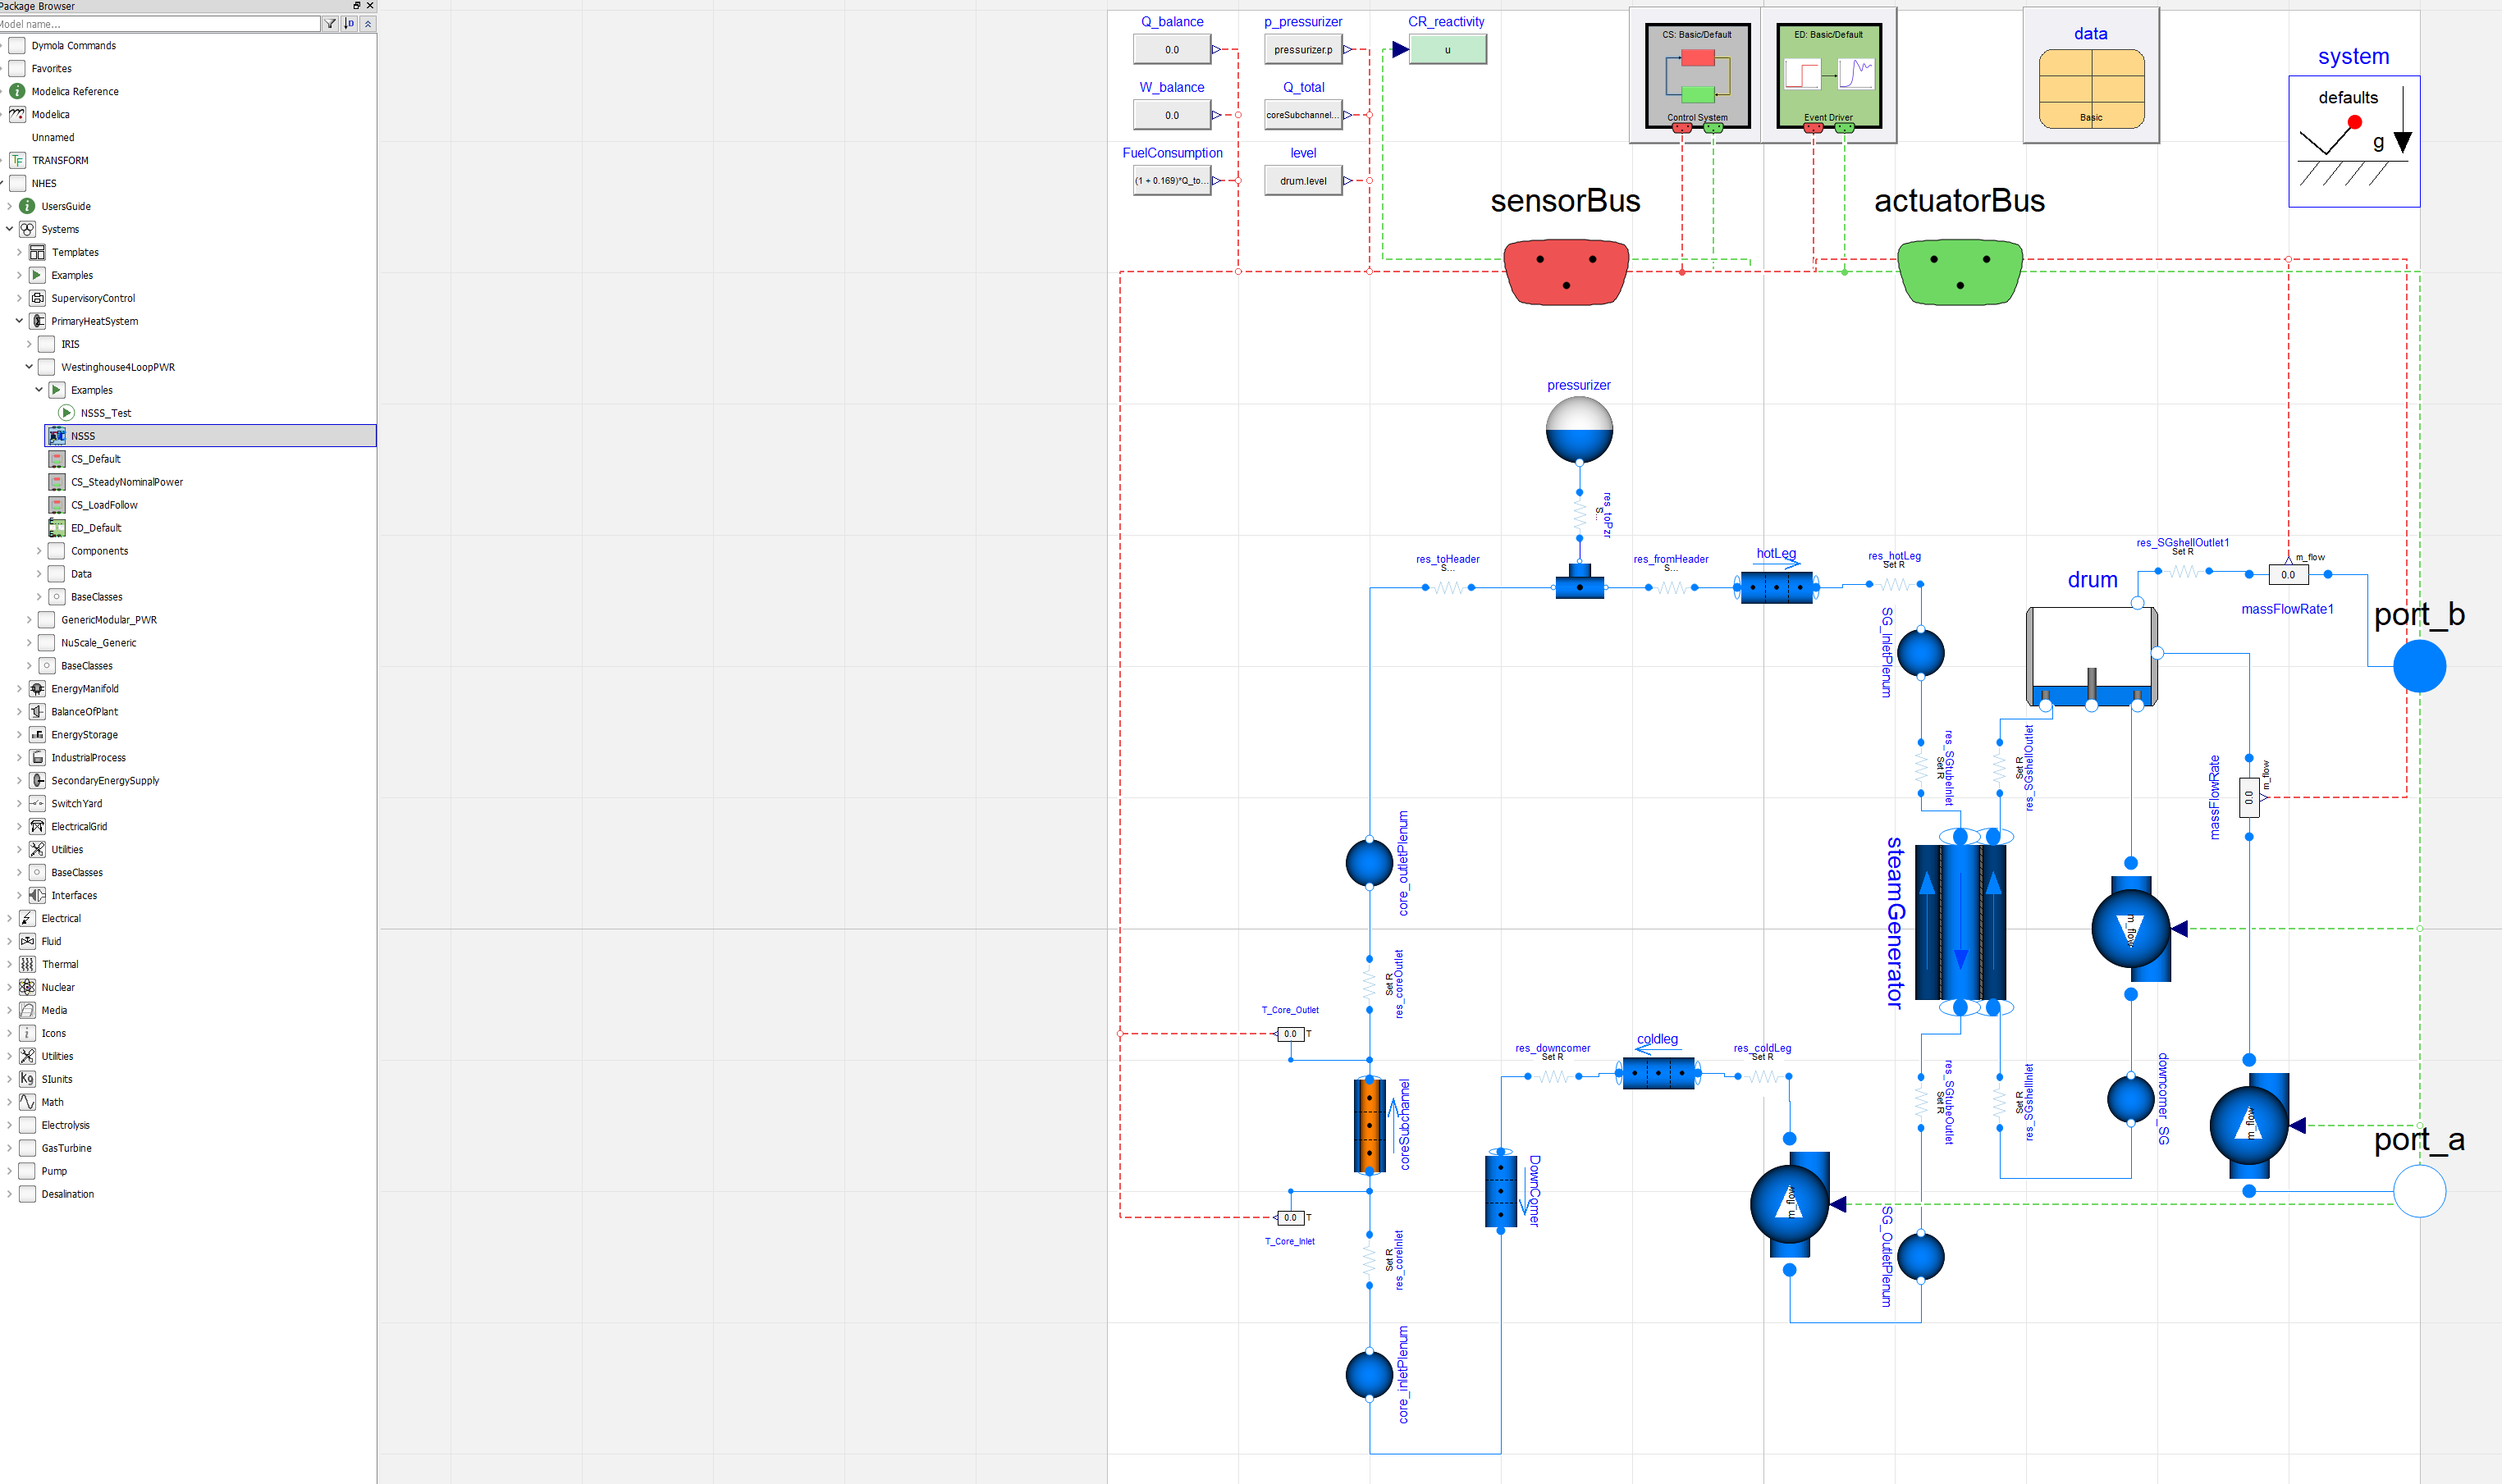
\includegraphics[width=\linewidth]{pics/Sub_System_Dummy.png}
\caption{Subsystem for the Westinghouse-4 Loop model.}
\label{Westinghouse 4-loop}
\end{figure}


\begin{figure}[hbtp]
\centering
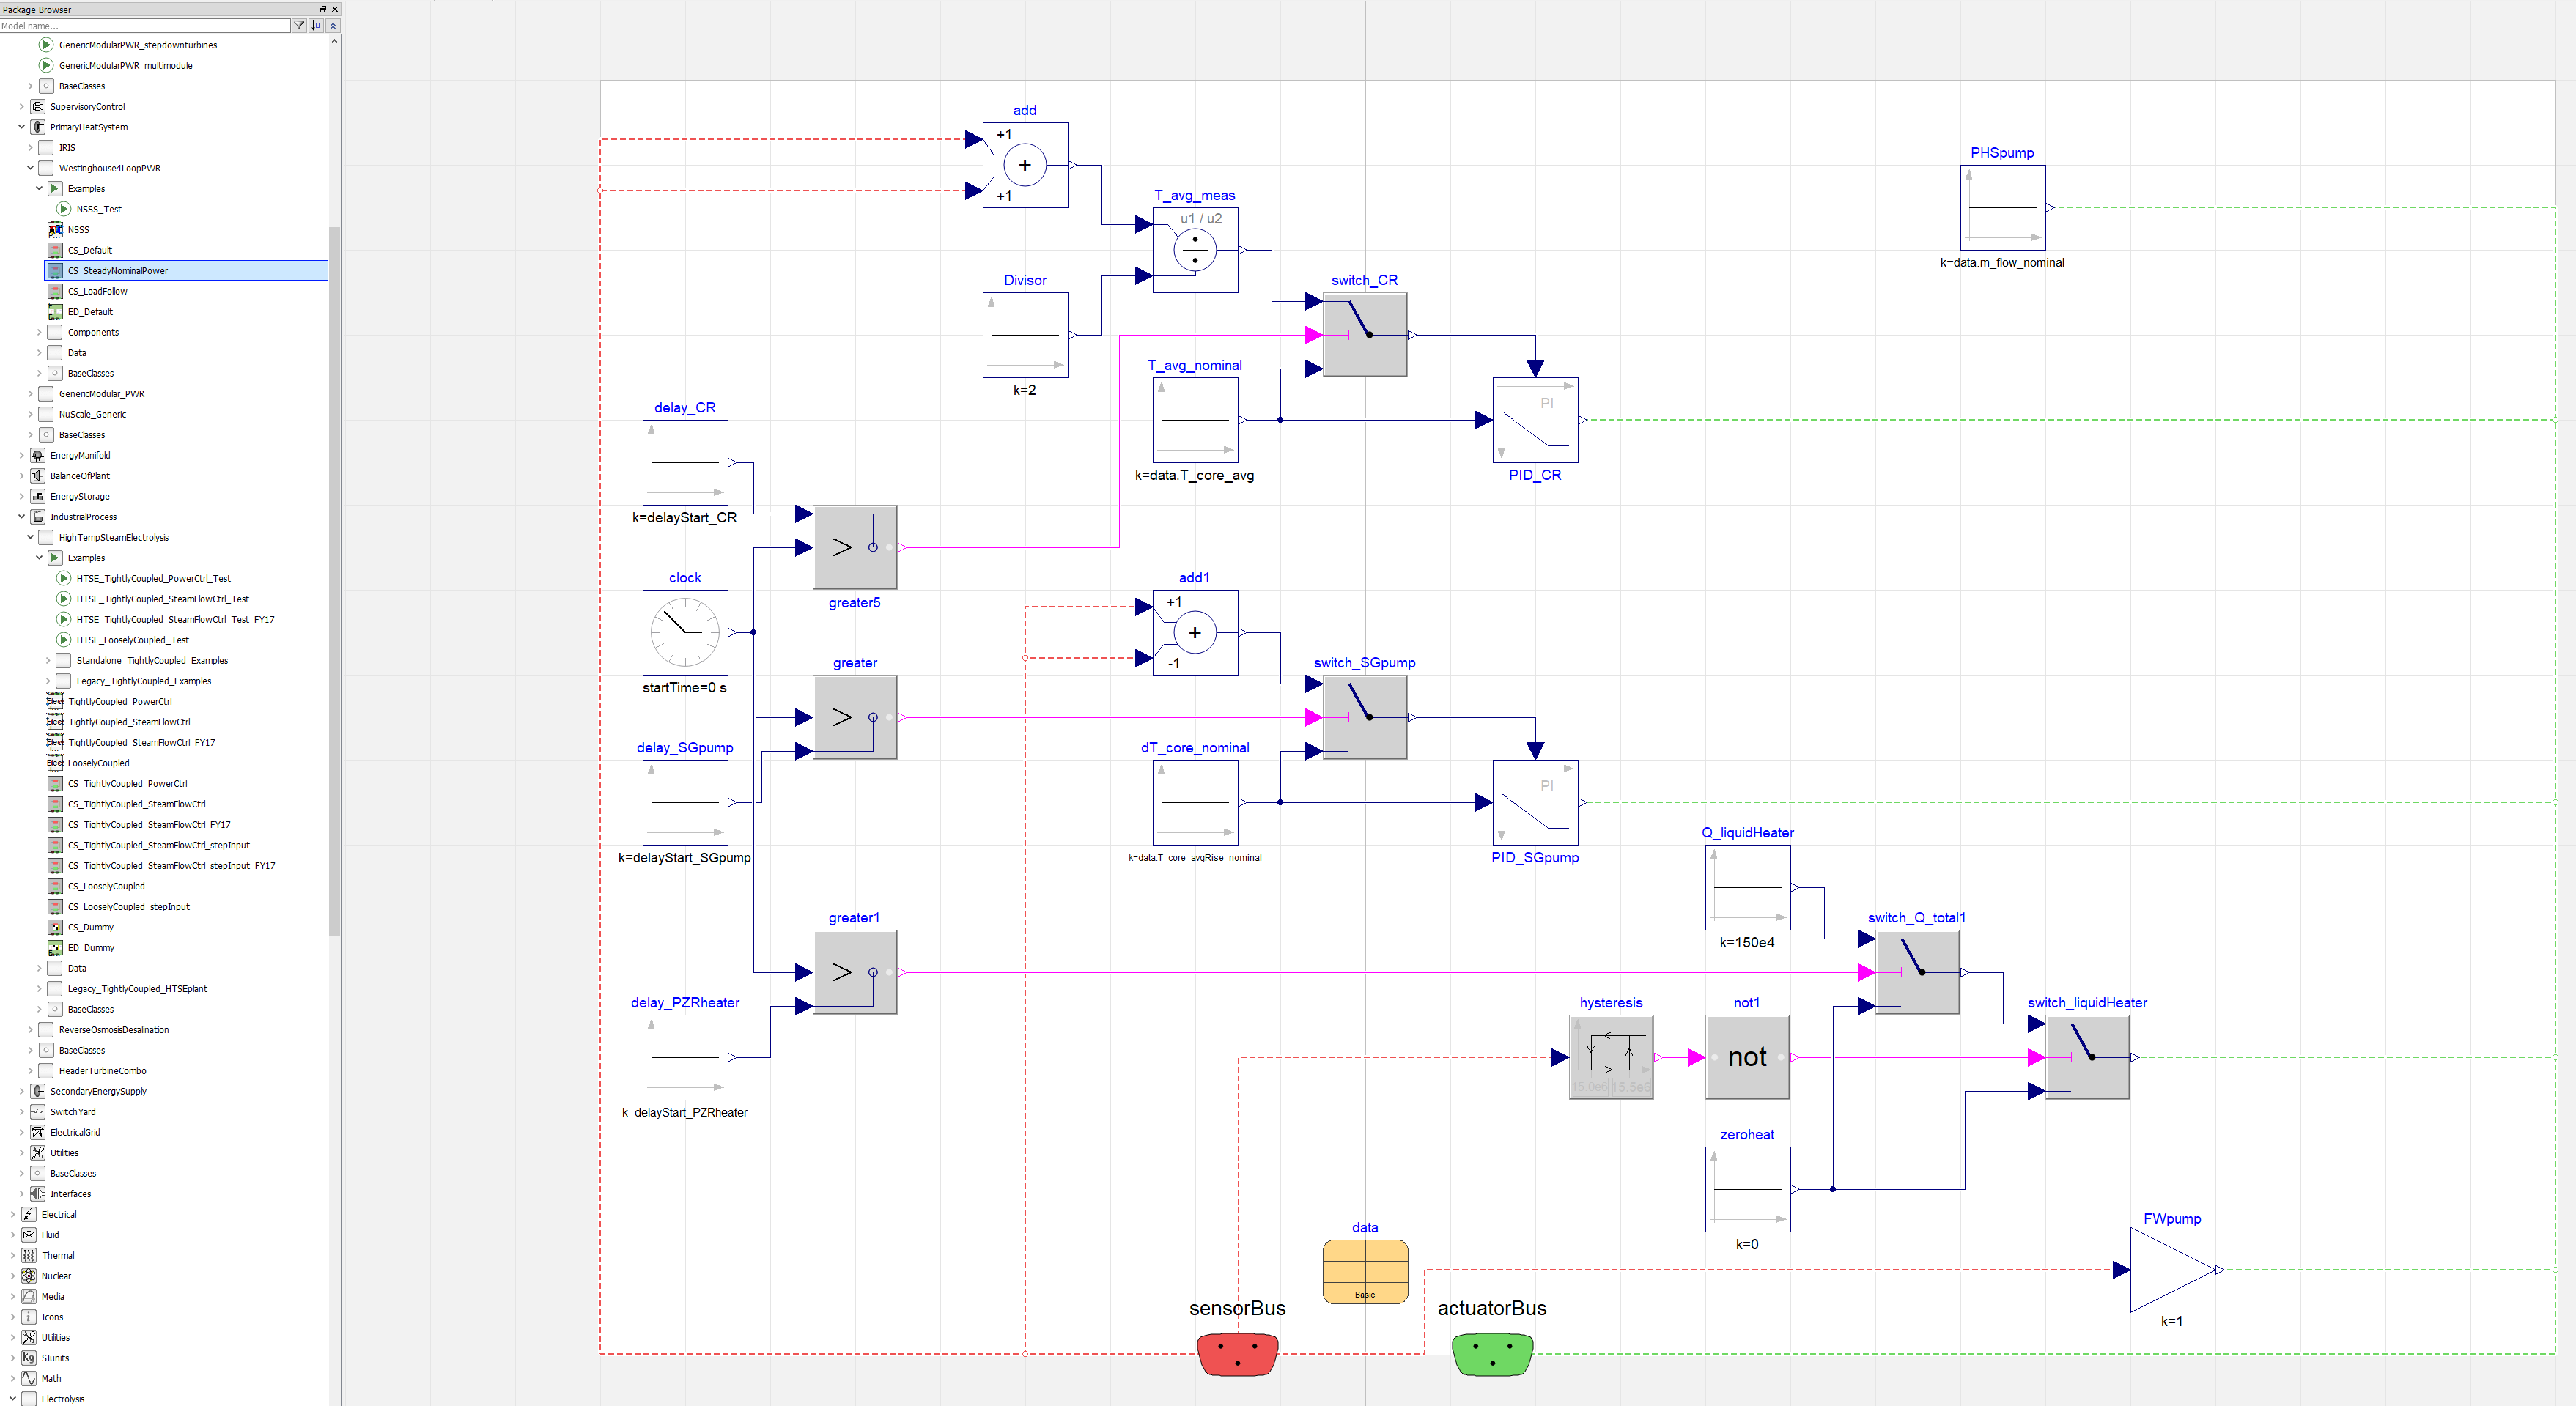
\includegraphics[width=\linewidth]{pics/Westinghouse_Control_picture.png}
\caption{Control System (CS) for the Westinghouse 4 Loop model}
\label{Control System}
\end{figure}

Assuming the user is creating a new package with new components specific to the model it is best to include those models with a “components” folder in the subpackage containing the “BaseClasses” folder. The Data folder is typically where the main data structures in terms of “records” of kept for the process model. Records are files that are intended to be used as an input deck to the main model for use as a set of “parameters” the components will read from. The ED\textunderscore dummy file within the \textit{Subsystem\textunderscore Specific} category is the Event Driver file and is rarely used and can be ignored from a user perspective.

\subsubsection{Modifying Existing Models for Specific Runs}
A starting point from which a user can begin model development and analysis is from an existing Example model. To properly edit the \textit{Examples} within the hybrid repository while still maintaining the regression system one needs to create a duplicate model of the example file that is to be edited. This can be done by right clicking on the file as shown below and creating a duplicate class.

\begin{figure}[hbtp]
\centering
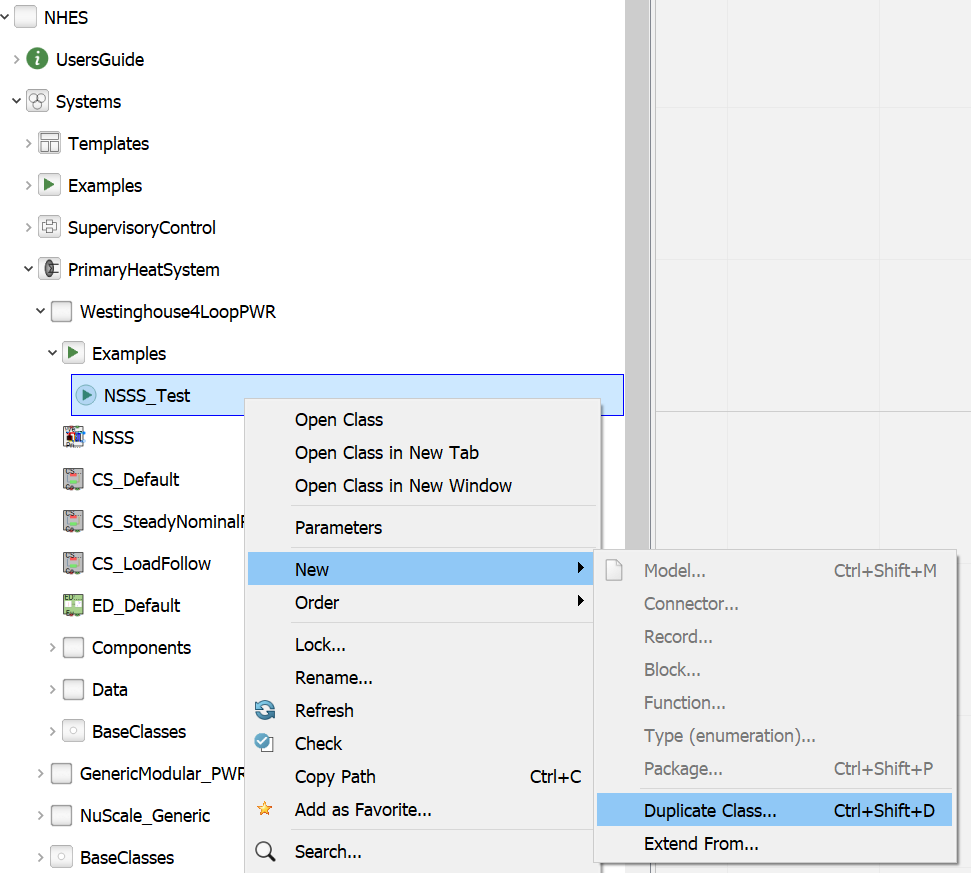
\includegraphics[width=\linewidth]{pics/DuplicateClass.png}
\caption{Creating a duplicate class for model runs.}
\label{Duplicate Class}
\end{figure}

This file will the be placed in the Examples folder where edits can be made to it for new and unique runs. This includes things such as new control schemes, sizing, timeruns, etc..

\subsection{Configuring Existing Models into Integrated Energy Systems}
Each subsystem of the Integrated Energy Systems is inherently interesting on its own and large spans of time can be spent researching and fine tuning them independently. However, the developer team is aware that in the evolving energy landscape, and to the extent users will come across this repository, that integrated energy systems are the primary focus.

This focus includes systems that involve the distribution of heat and electrical energy among several subsystems and the control schemes utilized to accomplish this. Therefore, this section seeks to provide an introductory understanding of how to connect subsystems together within the Hybrid repository. To accomplish this the NuScale\textunderscore Coupling\textunderscore Test Example will be created starting from the GenericModularPWR\textunderscore park system.

\begin{figure}[hbtp]
\centering
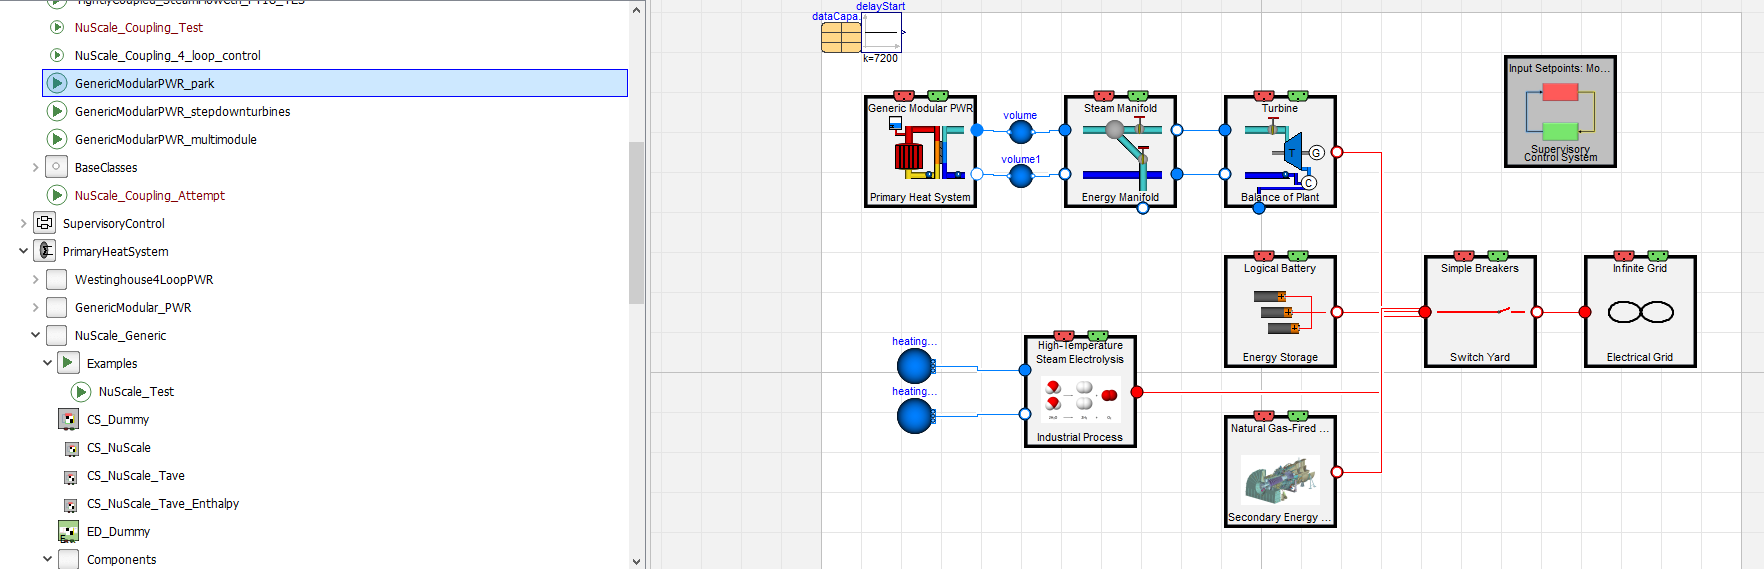
\includegraphics[width=\linewidth]{pics/Modular_Park_Start.png}
\caption{Initial Integrated Energy System Starting Point}
\label{modular park}
\end{figure}

The first step is to take a similar example that has the Supervisory Control System in the top level. In this case the GenericModularPWR\textunderscore park was used. A duplicate class was created and all the components aside the Steam Manifold, Turbine, Simple Breakers, infinite grid, supervisory control system, delay start, and data capacity were removed. See below.

\begin{figure}[hbtp]
\centering
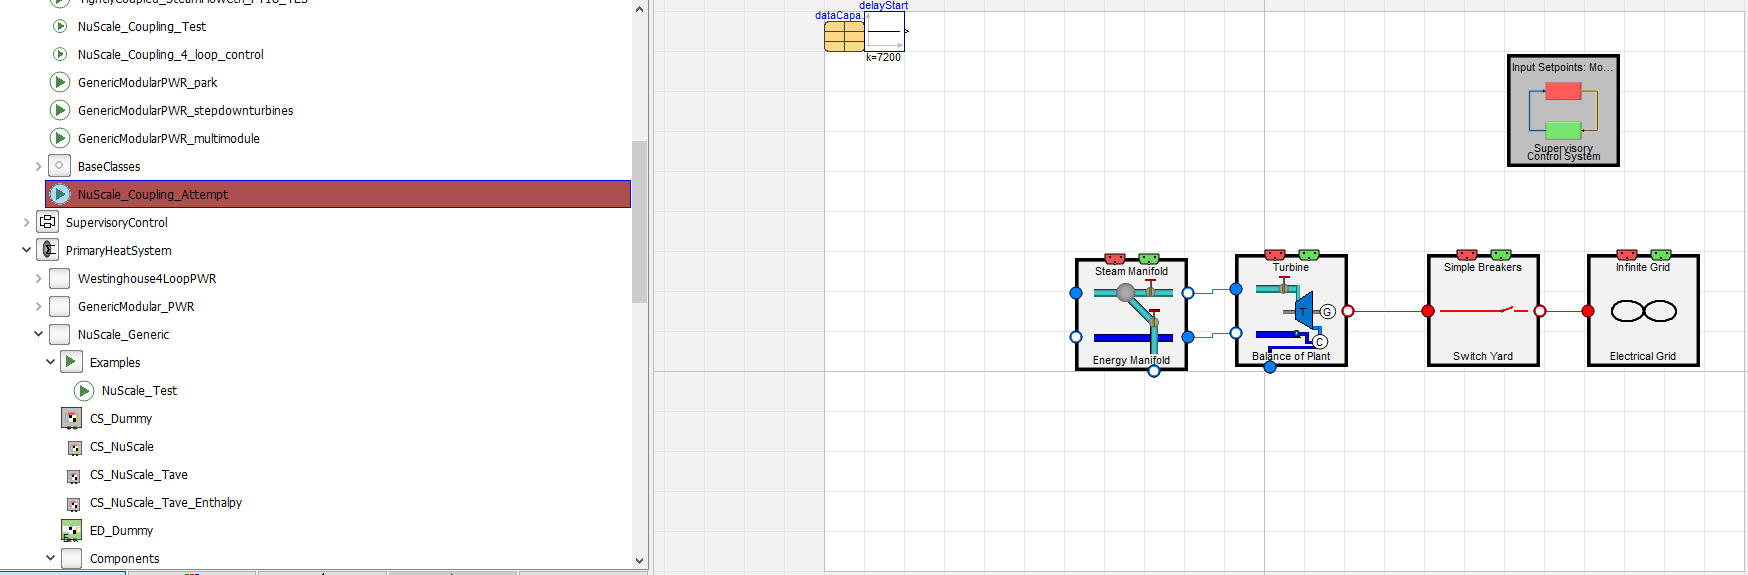
\includegraphics[width=\linewidth]{pics/CouplingCreation.png}
\caption{Rearrangement of Initial Energy System}
\label{coupling park}
\end{figure}

Then the primary side of the NuScale was added in this case the \textit{NuScale\textunderscore Taveprogram} version of the NuScale primary unit.

\begin{figure}[hbtp]
\centering
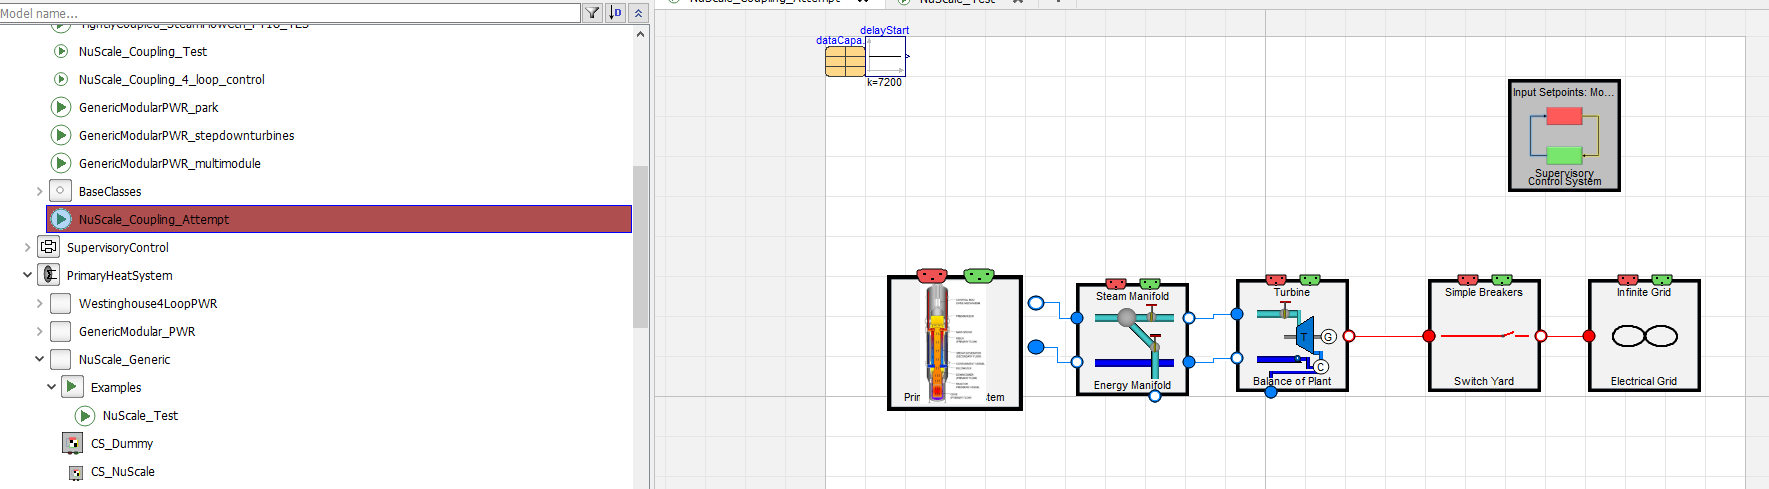
\includegraphics[width=\linewidth]{pics/CouplingCreation_2.png}
\caption{Creation of NuScale Energy System}
\label{NuScale park}
\end{figure}

Then from this point it is a matter of telling the systems what control schemes to use. For this system the reactor operates to meet a certain primary system average temperature in accordance with the turbine output. To input this the control system: PrimaryHeatSystem.NuScaleGeneric.\\ CS\textunderscore NuScale\textunderscore Tave was used with input:
W\textunderscore turbine = BOP.powerSensor.power and W\textunderscore Setpoint  =  SC.W\textunderscore totalSetpoint\textunderscore BOP, see Figure \ref{primary controller settings}.  And the turbine control scheme is modified to reflect a once through system type control strategy where the turbine control valve operates to meet a constant pressure in the turbine, Figure \ref{Turbine Control Settings}. While it is noted that is not the official control strategy strictly speaking for the NuScale system nor is it the one used in load following scenarios in the hybrid repository, it does provide a baseline for which to control the system and modifications can be made from this point.  The power setpoints in the BalanceOfPlant.Turbine.CS\textunderscore OTSG\textunderscore Pressure control module are 160MW for both Reactor\textunderscore Power and Nominal\textunderscore Power while p\textunderscore nominal parameter is set to BOP.port\textunderscore a\textunderscore nominal.p to ensure a single parameter value is carried throughout the system. Additionally, W\textunderscore totalSetpoint is set to SC.W\textunderscore totalSetpoint\textunderscore BOP, Figure \ref{Turbine Control Settings}.

\begin{figure}[hbtp]
\centering
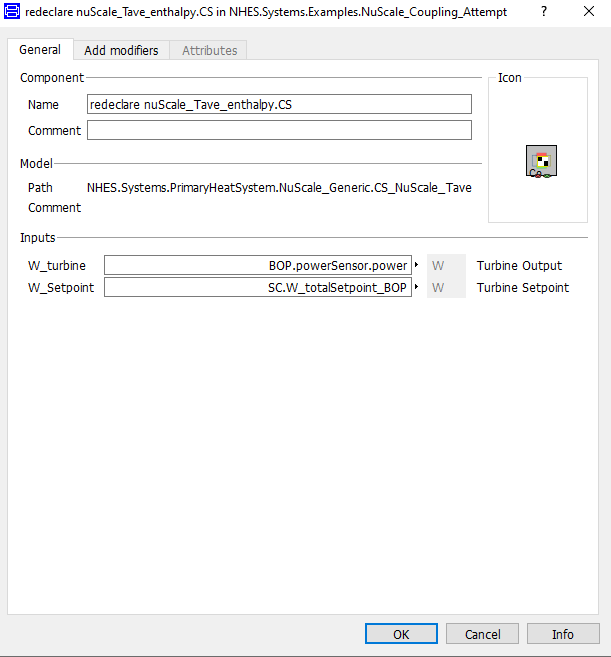
\includegraphics[width=\linewidth]{pics/primary_controller_settings.png}
\caption{Primary System Controller Settings}
\label{primary controller settings}
\end{figure}


\begin{figure}[hbtp]
\centering
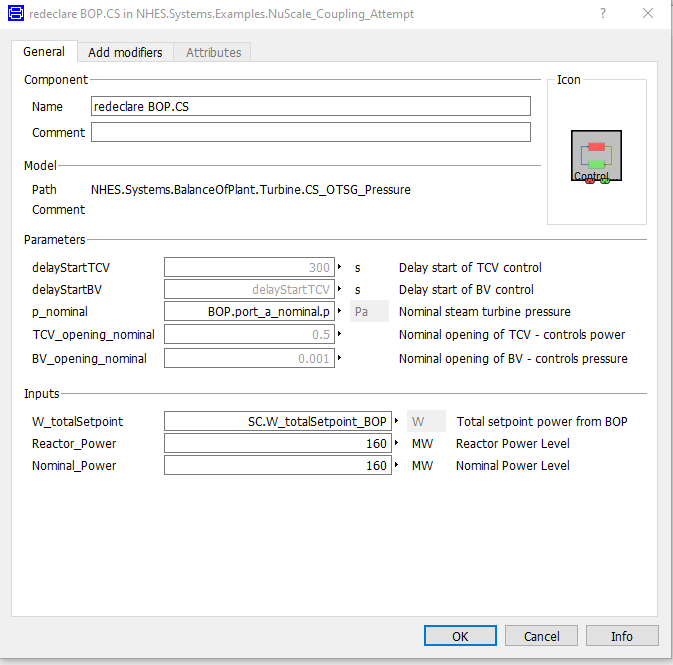
\includegraphics[width=\linewidth]{pics/BOP_settings.png}
\caption{Turbine Control Settings}
\label{Turbine Control Settings}
\end{figure}

To complete the construction of the model the systems need to match on the boundaries.  To do this the values from the primary heat system need to be transferred to the Steam Manifold under the nominal values tab, Figure \ref{Port a Nominal Values} and \ref{port B Nominal Values}.

\begin{figure}[hbtp]
\centering
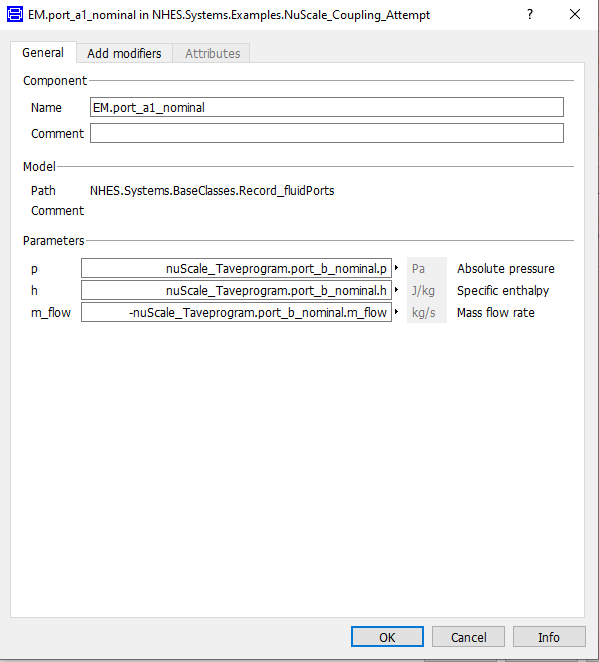
\includegraphics[width=\linewidth]{pics/Nominal_Values_BOP.png}
\caption{Port a Boundary Values of the Energy Manifold}
\label{Port a Nominal Values}
\end{figure}

\begin{figure}[hbtp]
\centering
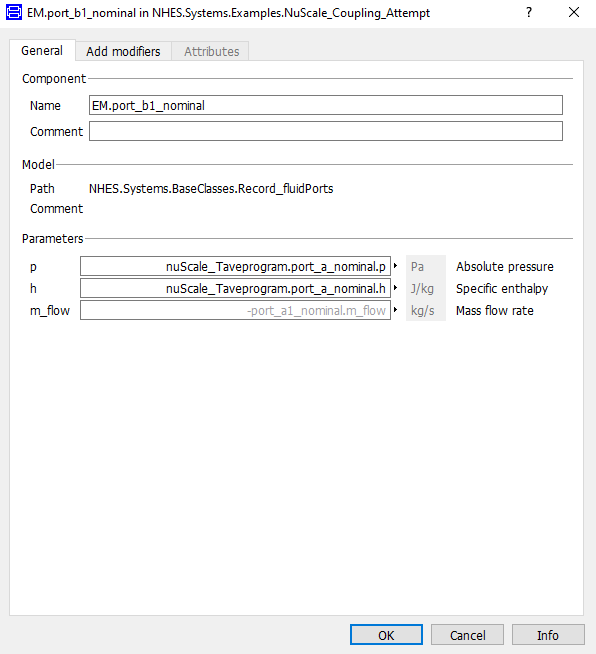
\includegraphics[width=\linewidth]{pics/Manifold_Nominal_b.png}
\caption{Port b Nominal Values of the Energy Manifold }
\label{port B Nominal Values}
\end{figure}

\subsection{Test Creation}
To create a regression test once a user develops an example test in the Dymola NHES library can be accomplished through a couple of settings. In the Dymola simulation setup tab in the output tab uncheck the store at variable events box. Then click store in model button and check the output box, click ok, then click ok again, then Save the model. Example settings are shown in Figure \ref{mat file settings}.


%\begin{figure}[hbtp]
%\caption{dfgsg}
%\centering
%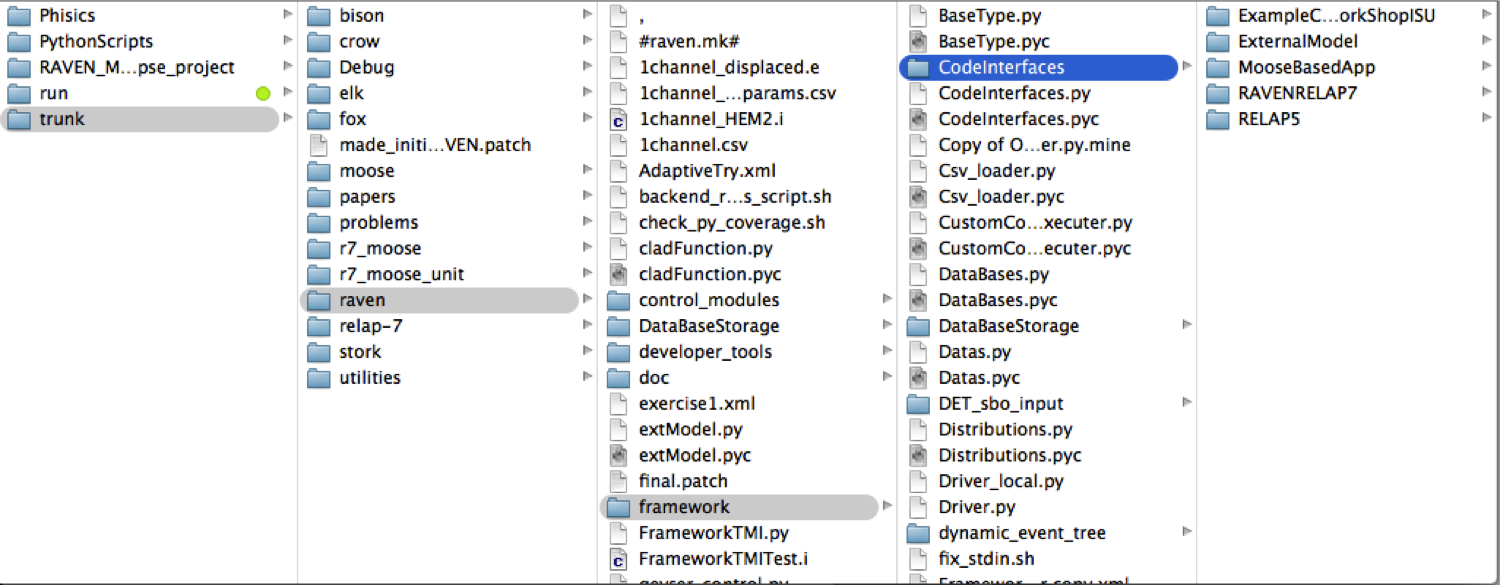
\includegraphics[width=\linewidth]{pics/CodeInterfaceLocation.png}
%\end{figure}


\begin{figure}[hbtp]
\centering
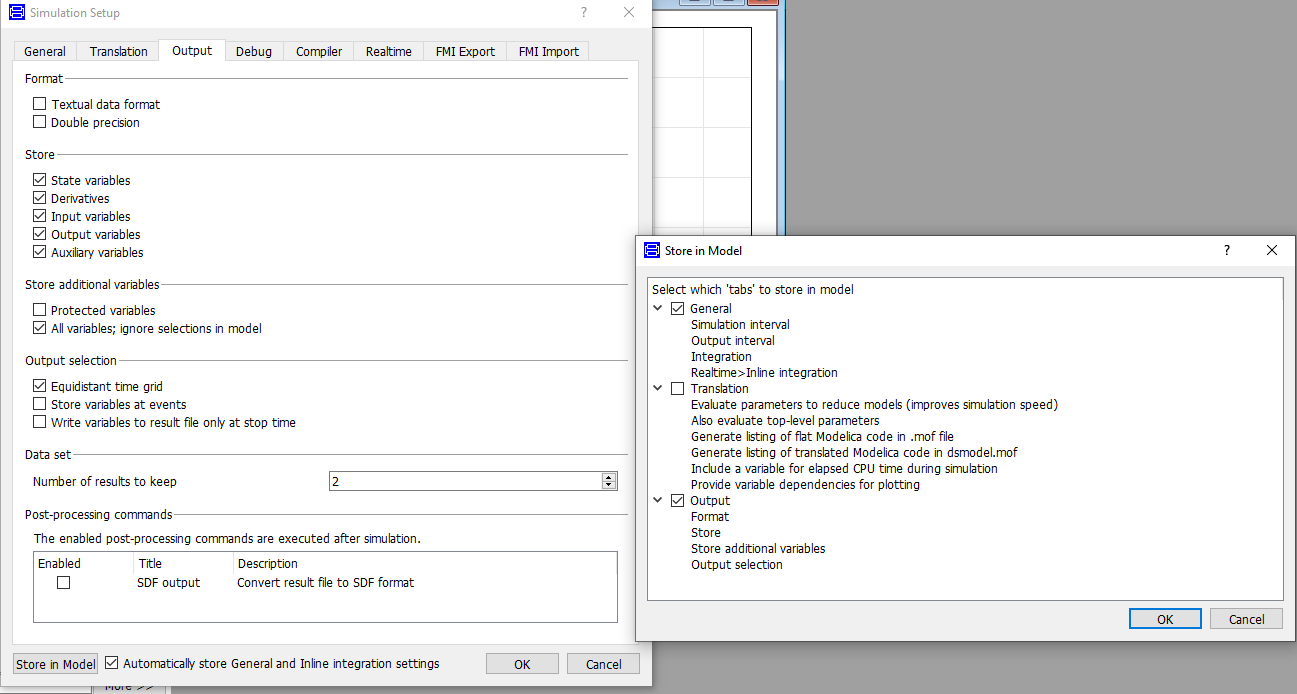
\includegraphics[width=\linewidth]{pics/Test_Creation.png}
\caption{Settings to Create a proper mat file for a gold folder test}
\label{mat file settings}
\end{figure}
In the simulateModel command one of the following two flags is required. Either "\textit{numberOfIntervals}" or "\textit{OutputInterval}". numberOfIntervals tells dymola how many output intervals to make. OutputInterval tells dymola at what timestep interval should an output be present for comparison. The .mat file in the gold folder will need to be run using the same simulateModel command that is present in the .mos file being created.

These can be selected in the Simulation Setup tab of the Dymola GUI, Figure \ref{Interval Setup}, and should carry down to the command you copy and paste in the .mos file. An example is shown below of the simulation setup tab.

\begin{figure}[hbtp]
\centering
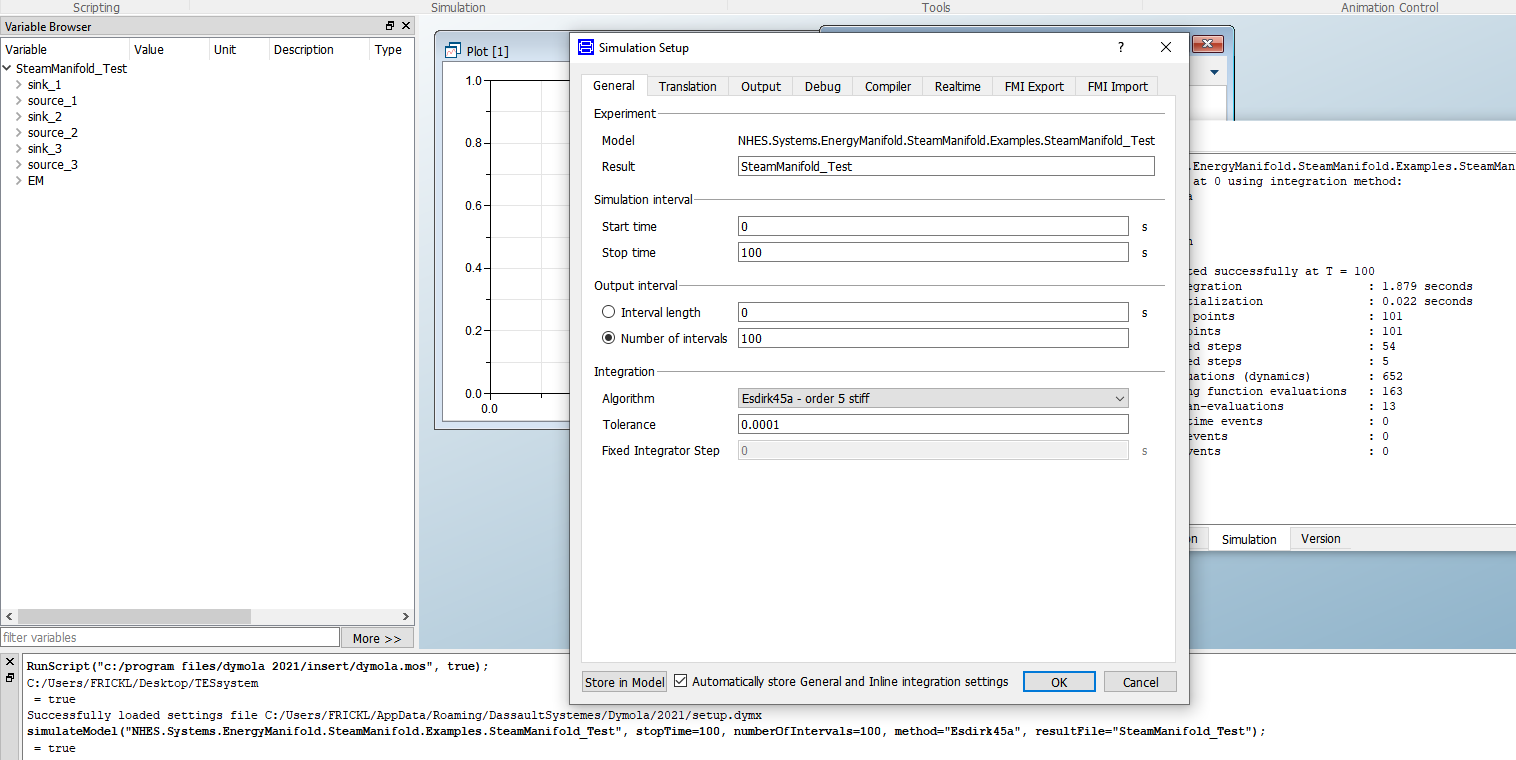
\includegraphics[width=\linewidth]{pics/Regression_picture.png}
\caption{Simulation Setup}
\label{Interval Setup}
\end{figure}

Then run the simulation, (ideally a test should take less than 100 seconds). On the simulation tab in the command line copy the simulation command. Example below:

\begin{lstlisting}[language=bash, basicstyle=\small]
simulateModel("NHES.Systems.EnergyManifold.SteamManifold.
Examples.SteamManifold_Test", stopTime=100, numberOfIntervals=100,
method="Esdirk45a", resultFile="SteamManifold_Test");
\end{lstlisting}

This command should then be added to a file and named something like Test\textunderscore Example.mos. The command can be found in the Simulation Setup tab of the Dymola GUI once you hit simulate

Then in folder /path/to/hybrid/hybrid/tests/dymola\textunderscore tests create a folder named Test\textunderscore YourModel.

Create a \textit{gold} folder in the new folder, drop the .mat file from your simulation that is named resultFile="SteamManifold\textunderscore Test" from your simulateModel command into the gold folder. The .mat file is created in your working directory in Dymola. Then in the main Test\textunderscore YourModel folder drop the Test\textunderscore Example.mos file and create a tests file open it up and place the following in it:


\begin{lstlisting}[language=bash, basicstyle=\small]
[Tests]
 [./]
  type = 'HYBRIDTester'
  input = 'Test_Example.mos'
  workingDir = '.'
  output = 'SteamManifold_Test.mat'
  dymola_mats = 'SteamManifold_Test.mat'  
  rel_err = 0.001
 [../]
[]
\end{lstlisting}

where SteamManifold\textunderscore Test.mat should be your result .mat file name, rel\textunderscore error is the amount of error allowed between the gold file and the regression test output, and Test\textunderscore Example.mos is the run script created.

\subsection{Advanced Test File Options utilized for complex models}
For complex models the initialization phase of a simulation can take the Modelica solvers a significant amount of time to find an initialization point. This occurs due to the highly nonlinear nature of the underlying physical equations.  A way to avoid such situations is to provide a restart file to bypass the initialization phase of the simulation. A restart file is automatically created at the end of each simulation as the dsfin.txt file created in the folder where the simulation is run. This file includes the final values of the previous simulation from which the new model can restart.   Move this file to the gold folder for your new testing system.
Once this file is created it can then be loaded automatically via the continue button in Modelica under the Simulation Tab. Select $Continue \rightarrow  Import Initial  \rightarrow  dsfin.txt  $. See Figure \ref{import Initial}.

\begin{figure}[hbtp]
\centering
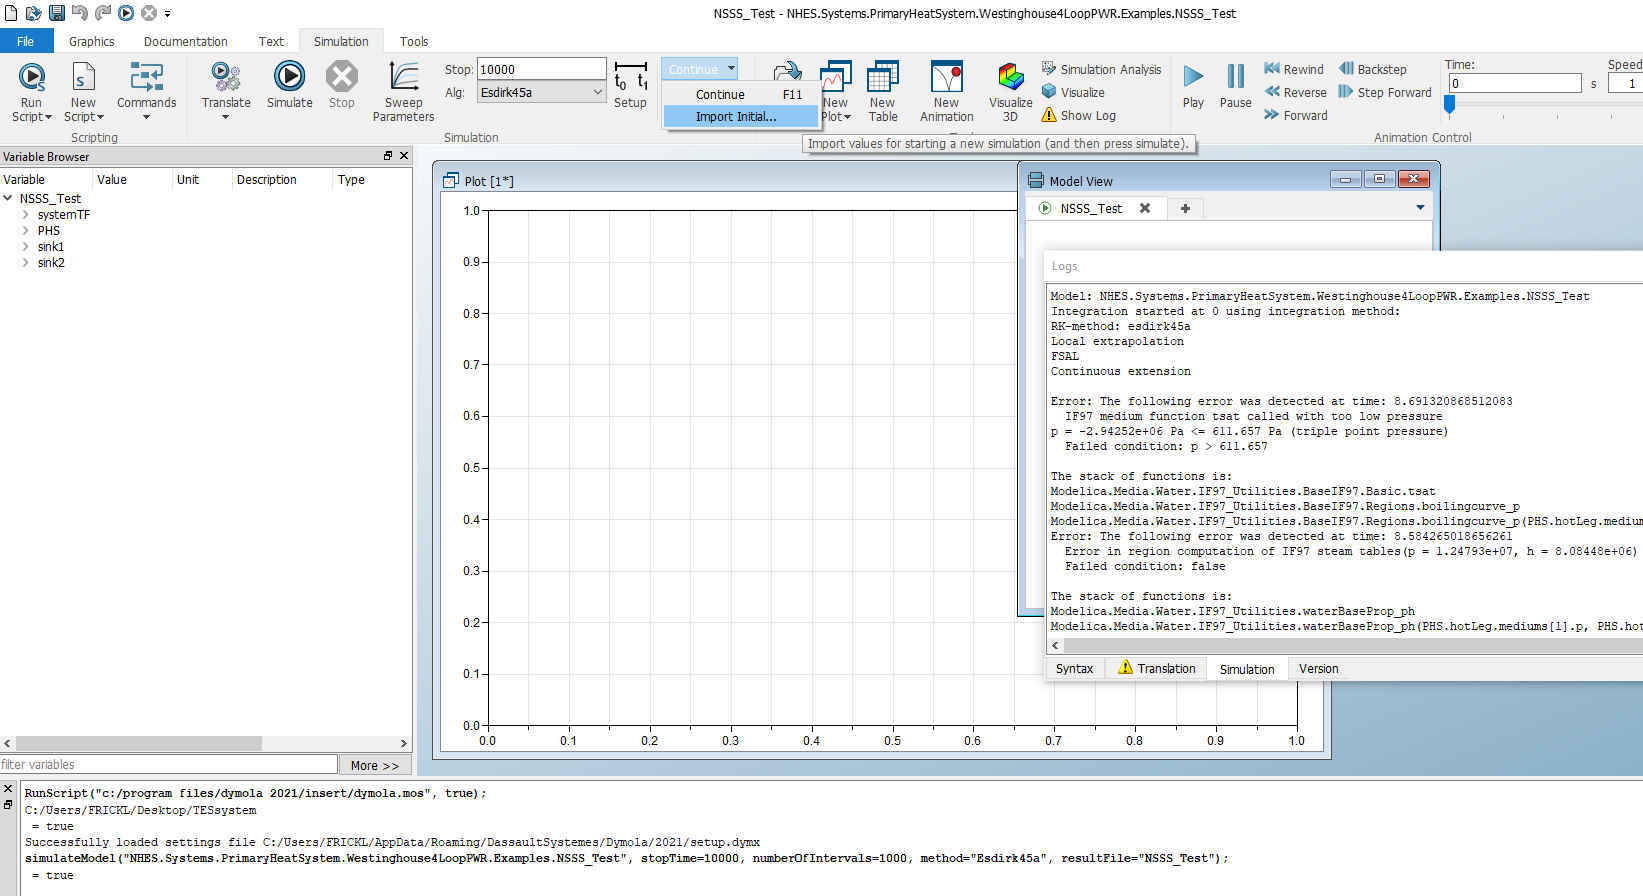
\includegraphics[width=\linewidth]{pics/Import_Initial.png}
\caption{Import Initial conditions from a previously run simulation}
\label{import Initial}
\end{figure}

Then once the dsfin.txt file is loaded go into the Setup tab and move the time back to start from zero and the end time to the desired simulation point for the test, shown in Figure \ref{Simulation Time Realignment}. This is necessary since Dymola assumes the user wants to restart the simulation from where it ended in time as well. This is not the case for the test. Instead the goal is to skip the initialization phase of the simulation and provide a clean solution with which to compare.

\begin{figure}[hbtp]
\centering
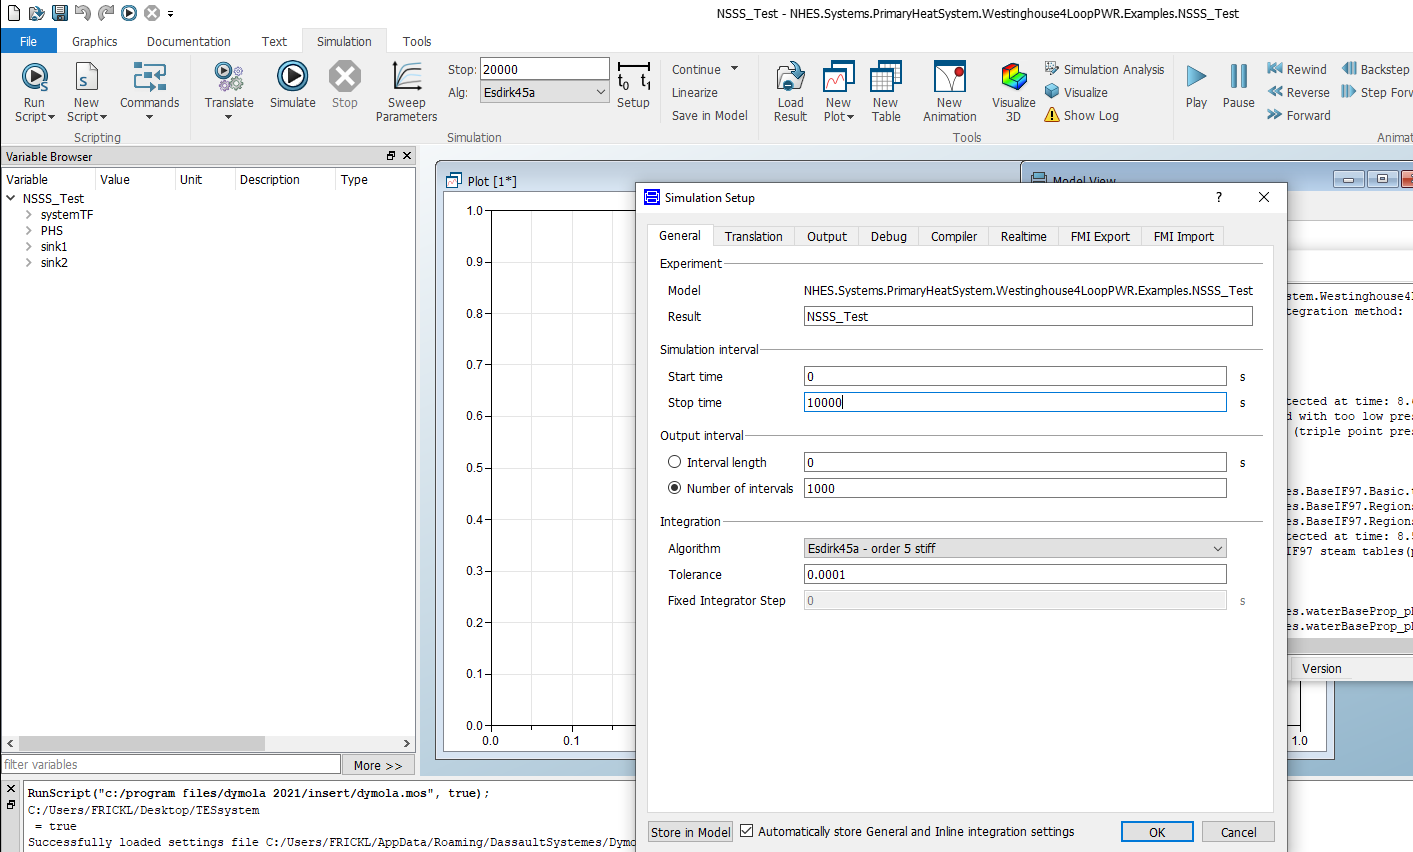
\includegraphics[width=\linewidth]{pics/Move_back_time.png}
\caption{Realign the Simulation Time}
\label{Simulation Time Realignment}
\end{figure}

Simulate this model and save the result file, in this example “NSSS\textunderscore Test.mat” and place it into the gold folder of the testing system. Additionally, copy and paste the simulateModel command that is in the Dymola GUI as the last line of your .mos script file for the test. The first two lines should be translateModel to make sure the right model is loaded into the equation set, followed by the importInitial command that loads all the values into the translated Model. The final command should be the simulateModel command.
The .mos file should look something like what is shown below.

\begin{lstlisting}[language=bash, basicstyle=\small]
translateModel("NHES.Systems.PrimaryHeatSystem.Westinghouse4LoopPWR
.Examples.NSSS_Test");

importInitial("./gold/dsfinal.txt");

simulateModel("NHES.Systems.PrimaryHeatSystem.Westinghouse4LoopPWR.
Examples.NSSS_Test", stopTime=10000, numberOfIntervals=250,
method="Esdirk45a", resultFile="NSSS_Test");
\end{lstlisting}